\documentclass[11pt]{article}
\usepackage[utf8]{inputenc} % Para caracteres en espa�ol
\usepackage{amsmath,amsthm,amsfonts,amssymb,amscd}
\usepackage{multirow,booktabs}
\usepackage[table]{xcolor}
\usepackage{fullpage}
\usepackage{lastpage}
\usepackage{enumitem}
\usepackage{multicol}
\usepackage{fancyhdr}
\usepackage{mathrsfs}
\usepackage{wrapfig}
\usepackage{setspace}
\usepackage{esvect}
\usepackage{calc}
\usepackage{multicol}
\usepackage{cancel}
\usepackage{graphicx}
\graphicspath{ {pictures/} }
\usepackage[retainorgcmds]{IEEEtrantools}
\usepackage[margin=3cm]{geometry}
\usepackage{amsmath}
\newlength{\tabcont}
\setlength{\parindent}{0.0in}
\setlength{\parskip}{0.05in}
\usepackage{empheq}
\usepackage{framed}
\usepackage[most]{tcolorbox}
\usepackage{xcolor}
\colorlet{shadecolor}{orange!15}
\parindent 0in
\parskip 12pt
\geometry{margin=1in, headsep=0.25in}
\theoremstyle{definition}
\newtheorem{defn}{Definition}
\newtheorem{reg}{Rule}
\newtheorem{exer}{Exercise}
\newtheorem{note}{Note}
\newcommand{\volume}{{\ooalign{\hfil$V$\hfil\cr\kern0.08em--\hfil\cr}}}
\newcommand{\parr}{\mathbin{\|}} % Parralel Symbol
\begin{document}
\setcounter{section}{2}
\setcounter{page}{9}
\setcounter{equation}{16}
%\definecolor{babyblue}{rgb}{0.54, 0.81, 0.94}
\definecolor{babyblueeyes}{rgb}{0.63, 0.79, 0.95}
\definecolor{babyblue}{rgb}{0.69, 0.88, 0.9}

 \pagestyle{fancy}
\fancyhf{}
\rhead{Section 4:  Kinetic Theory}
\rfoot{Page \thepage}
\thispagestyle{empty}


\begin{center}
{\LARGE \bf Section 4:  Kinetic Theory}\\
{\large AE435}\\
Spring 2018
\end{center}
\vspace{5mm}
\section{Velocity Distribution Function}

Not all particles move with the same velocity. Also, the
velocity of a particle doesn't remain the same over time.
We need a statistical way to describe this; this the velocity
distribution function.
%VDP a statistical way to describe the velocity of the particles in a system. 
\begin{center}
\vspace{25mm}
\end{center}
\tableofcontents
\newpage
%%%%%%%%%%%%%%%%%%%%%%%%%%%%%%%%%%%%%%%%%%%%%%%%%%%%%%%%
%%%%%%%%%%%%%%%                           SECTION 1                                     %%%%%%%%%%%%%%%
%%%%%%%%%%%%%%%%%%%%%%%%%%%%%%%%%%%%%%%%%%%%%%%%%%%%%%%%
\subsection{Mass Distribution Function}
To illustrate this idea of distribution function, consider mass density. Essentially what the mass distribution function expresses is a distribution across physical space. A change in the density of the gas in physical space. We will make the analogy of distribution in physical space and distribution in velocity space.
\begin{center}
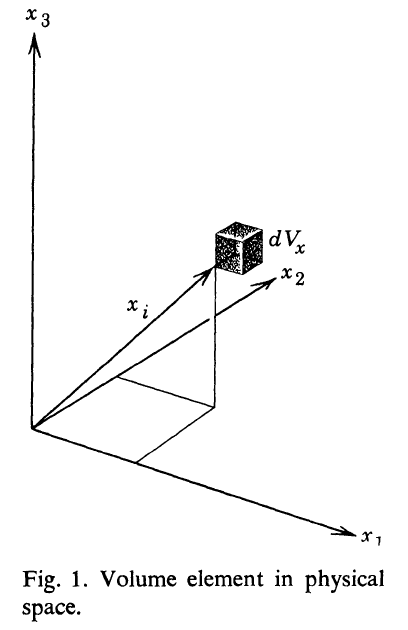
\includegraphics[width=10cm,height=10cm]{1.png}
\end{center}

Consider a gas of N particles with mass m in a volume V.

The density is:
\begin{equation}
\begin{aligned}
\rho = m \frac{N}{\volume} = mn
\end{aligned}
\end{equation}

If the gas is nonuniform, the density in a differential %not the same everywhere
volume
\begin{equation*}
\begin{aligned}
\mathrm{d}\volume_x = \mathrm{d}x_1\, \mathrm{d}x_2\, \mathrm{d}x_3
\end{aligned}
\end{equation*}
At a position vector
\begin{equation*}
\begin{aligned}
\vv{x}_i = \begin{bmatrix}x_1 & x_2 & x_3\end{bmatrix}
\end{aligned}
\end{equation*}
then the density at that location is:
\begin{equation}
\begin{aligned}
\rho(\vv{x}_i) = \lim_{\Delta \volume_x \rightarrow 0} \, m \, \frac{\Delta N}{\Delta \volume_x}
\end{aligned}
\end{equation}
\newpage
We still operate under the assumption that the volume contains a large number of particles.
Note that this assumes that $\Delta \volume_x$ is large enough to
contain a large number of particles. Since the particle
mass doesn't change, 
\begin{equation*}
\begin{aligned}
\rho(\vv{x}_i) = m \, \lim_{\Delta \volume_x \rightarrow 0} \, \frac{\Delta N}{\Delta \volume_x}
\end{aligned}
\end{equation*}
Which we can write as:
\begin{equation}
\begin{aligned}
\rho(\vv{x}_i) = m \, n(\vv{x}_i)
\end{aligned}
\end{equation}

Meaning that the mass density can be different depending on where we stand in physical space.

The function $n(\vv{x}_i)$ gives the number of particles per
unit volume as a function of position; a.k.a. a "position
distribution function"

The number of particles in the differential volume $\mathrm{d}\volume_x$
is
\begin{equation*}
\begin{aligned}
\mathrm{d}N = n(\vv{x}_i) \, \mathrm{d}\volume_x
\end{aligned}
\end{equation*}
So the mass within that differential volume is
%position distribution function is an absolte, it gives you number at a specific loacation. Typically we work on it in a normalized form making it more of a probability density funcition
\begin{equation*}
\begin{aligned}
\mathrm{d}M = m \mathrm{d}N = \rho(\vv{x}_i) \, \mathrm{d}\volume_x
\end{aligned}
\end{equation*}
We can define a "normalized distribution function" as
\begin{equation}
\begin{aligned}
w(\vv{x}_i) = \frac{n(\vv{x}_i)}{N}
\end{aligned}
\end{equation}
Which is essentially just the percent of particles at position $x_i$

So that the total number of particles in $\mathrm{d}\volume_x$ is
\begin{equation}
\begin{aligned}
\mathrm{d}N = N \, w(\vv{x}_i) \, \mathrm{d}\volume_x
\end{aligned}
\end{equation}
This normalized distribution function can be interpreted
as a \textbf{probability density function}, that is, the probability
that a given randomly-chosen particle will be in $\mathrm{d}\volume_x$. In other words, it is the probability that a particle will be at a specific location. %probability that a particles will be at that location

Integrating over the entire volume,
\begin{equation*}
\begin{aligned}
\int_{\volume} \, w(\vv{x}_i) \mathrm{d}\volume_x = 1
\end{aligned}
\end{equation*}
%if we integrate over all volume, the probability of particle 
If we integrate over the entire volume, the probability that a particle within the volume is within the volume is 100\%. As expected.

We can generalize this idea to state:

A distribution function gives the concentration of some quantity per unit "volume" as a function of position in some kind of "space". 
% Here it was physical space, the number of particles in a given spacial volume within physical space. We can make the analogy now into a velocity distribution function. The number of particles that are within a volume and velocity space. How are the particles distributed across velocity space.
\newpage
%%%%%%%%%%%%%%%%%%%%%%%%%%%%%%%%%%%%%%%%%%%%%%%%%%%%%%%%
%%%%%%%%%%%%%%%                           SECTION 2                                     %%%%%%%%%%%%%%%
%%%%%%%%%%%%%%%%%%%%%%%%%%%%%%%%%%%%%%%%%%%%%%%%%%%%%%%%
\subsection{Velocity Distribution Function}
Now consider particle with velocity $\vv{c} = \begin{bmatrix}c_1 & c_2 & c_3\end{bmatrix}$

We can define a differential volume in this velocity space

\begin{center}
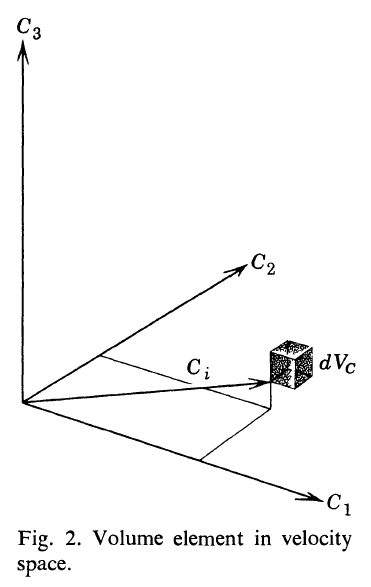
\includegraphics[width=10cm,height=10cm]{2.png}
\end{center}

Define local point density $F(\vv{c}_i)$ such that the number of
particles within velocity range: %the number of particles in the velocity grange
\begin{equation}
\begin{aligned}
c_1 \rightarrow c_1 + \mathrm{d}c_1 \\
c_2 \rightarrow c_2 + \mathrm{d}c_2 \\
c_3 \rightarrow c_3 + \mathrm{d}c_3 \\
\end{aligned}
\end{equation}
which we would write that as $F(\vv{c}_i) \mathrm{d}\volume_c$. This is the \textbf{velocity distribution
function}. Like the position distribution function $n(\vv{x}_i)$
you have to multiply by a volume to get a real quantity
(the number of particles). Essentially telling us  how particles are distributed across velocity space. %tells us how particles are distributed across velocity space, much like the position distributiuon function, we have to multiply by the volume to get the overall number of particls

Define a normalized velocity distribution function
\begin{equation}
\begin{aligned}
f(\vv{c}_i) = \frac{F(\vv{c}_i)}{N}
\end{aligned}
\end{equation}
%the fraction of particles that will be in the dvc elemet
This is the probability that a particle will be within the
specific velocity range. The number of particles within $\mathrm{d}\volume_c$ is
\begin{equation}
\begin{aligned}
\mathrm{d}N = N \, f(\vv{c}_i) \, \mathrm{d}\volume_c
\end{aligned}
\end{equation}
In terms of number density $n = \frac{N}{\volume}$
\begin{equation*}
\begin{aligned}
\mathrm{d}n = n \, f(\vv{c}_i) \, \mathrm{d}\volume_c
\end{aligned}
\end{equation*}
where the integral over all possible velocities is:
\begin{equation}
\begin{aligned}
\int_{-\infty}^{\infty} N \, f(\vv{c}_i) \, \mathrm{d}\volume_c = N \qquad \rightarrow \qquad \int_{-\infty}^{\infty} f(\vv{c}_i) \, \mathrm{d}\volume_c = 1
\end{aligned}
\end{equation}
Essentially saying that if you look over the entirety of velocity space, you will find N particles since that is the amount you have in the system. In other words, if we integrate over all of velocity space, the fraction of particles we will find is 1, 100\%.

The velocity distribution of particles is important for
determining average quantities. For instance, if we have
some quantity Q that depends on velocity $Q = Q(\vv{c}_i)$. The mean or expectation value of Q is then:

\begin{equation}
\begin{aligned}
\bar{Q} &= \frac{1}{N} \, \int_N Q \mathrm{d}N = \frac{1}{N} \, \int_{-\infty}^{\infty}  Q(\vv{c}_i) \, N \, f(\vv{c}_i) \, \mathrm{d}\volume_c \\ \\
&= \int_{-\infty}^{\infty}  Q(\vv{c}_i) \, f(\vv{c}_i) \, \mathrm{d}\volume_c \\ \\
<\vv{c}> &= \int_{-\infty}^{\infty} \vv{c} \, f(\vv{c}_i) \, \mathrm{d}\volume_c \\ \\
\end{aligned}
\end{equation}

Integrating over the distribution function. If Q is a velocity, then it is called taking the moment of the velocity distribution function.

For example if we were to do it of $<C>$ would be the first moment which is useful for finding the average collision rate, wether Q is the collision cross section which is tied with the particle velocity or if we want to find the average of some property that we are interested in finding, velocity, energy, over the entire system.
\newpage
%%%%%%%%%%%%%%%%%%%%%%%%%%%%%%%%%%%%%%%%%%%%%%%%%%%%%%%%
%%%%%%%%%%%%%%%                           SECTION 3                                     %%%%%%%%%%%%%%%
%%%%%%%%%%%%%%%%%%%%%%%%%%%%%%%%%%%%%%%%%%%%%%%%%%%%%%%%
\subsection{Maxwellian Velocity Distribution Function}
A gas at equilibrium has a special velocity distribution
function. Called the Maxwellian velocity distribution. This is not often the case for electric propulsion systems since plasmas are rarely in equilibrium.

Basic idea is that:
\begin{itemize}
\item Stationary velocity distribution
\item Collisions deplete and add to population at same rate % acollision that creates a certain outcome, cancels out with another collision. 
\item Thus, no net change.
\end{itemize}
Collision dynamics with simple billiard-ball model leads
to:
%mass is conserved in collsion. Subscript means its maxwellian
\begin{shaded}
\textbf{Maxwellian Velocity Distribution Function}
\begin{equation}
\begin{aligned}
f_M(\vv{c}_i) = \bigg(\frac{m}{2 \, \pi \, k \, T}\bigg)^{\frac{3}{2}} \, \exp \bigg[-\frac{m}{2 \, k \, T} \, (c_1^2 + c_2^2 + c_3^2)\bigg]
\end{aligned}
\end{equation}
where
\begin{equation*}
\begin{aligned}
m &= \text{Mass of Particle} \\
T &= \text{Temperature} \\
k &= \text{Boltzmann Constant} \\
\end{aligned}
\end{equation*}
\end{shaded}

We can break this into components along each axis

\begin{equation}
\begin{aligned}
\Xi_m (c_1) = \bigg(\frac{m}{2 \, \pi \, k \, T}\bigg)^{\frac{1}{2}} \, \exp \bigg[-\frac{m}{2 \, k \, T} \, c_1^2\bigg] \\ \\
\Xi_m (c_2) = \bigg(\frac{m}{2 \, \pi \, k \, T}\bigg)^{\frac{1}{2}} \, \exp \bigg[-\frac{m}{2 \, k \, T} \, c_2^2\bigg] \\ \\
\Xi_m (c_3) = \bigg(\frac{m}{2 \, \pi \, k \, T}\bigg)^{\frac{1}{2}} \, \exp \bigg[-\frac{m}{2 \, k \, T} \, c_3^2\bigg] \\ \\
\end{aligned}
\end{equation}

The probability that a particle will be within the velocity
space $\mathrm{d}\vv{c}_i = \mathrm{d}\volume_c$
\begin{equation}
\begin{aligned}
f_m(\vv{c}_i) \, \mathrm{d}c_1 \, \mathrm{d}c_2 \, \mathrm{d}c_3 = \Xi_m(c_1) \, \mathrm{d}c_1 \, \Xi_m(c_2) \, \mathrm{d}c_2 \, \Xi_m(c_3) \, \mathrm{d}c_3
\end{aligned}
\end{equation}
Which is simply the probability density function of the x, y and z component.

The Maxwellian VDF looks like this:
\begin{center}
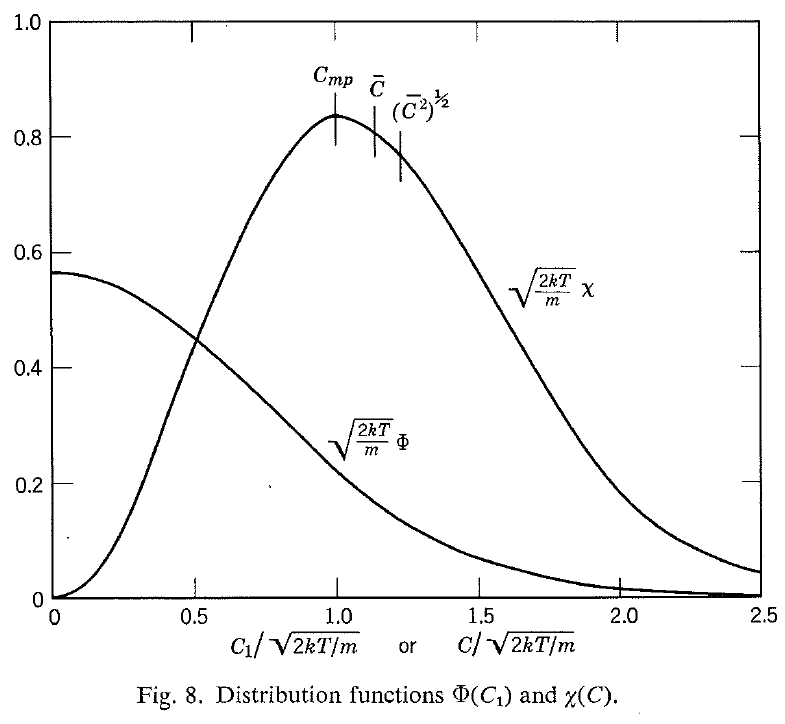
\includegraphics[scale=0.6]{3.png}
\end{center}
Shown in the plot, the smaller curve is the velocity distribution function. The negative x-axis isn't shown but it is symmetric. Particles can have negative velocity which is why we have this symmetry.

The largest probability is at $c_1 = 0$ which corresponds to
particles moving perpendicular to the $x_1$-axis with $\vv{c_i} \cdot \hat{x}_1 = 0$.

%The larger curve is the pseed distributation
We can transform the Maxwellian Velocity Distribution Function $f_m(\vv{c}_i)$ into a:
\begin{shaded}
\textbf{Maxwellian Speed Distribution Function}
\begin{equation}
\begin{aligned}
\chi_m(c)= 4 \pi  \bigg(\frac{m}{2 \, \pi \, k \, T}\bigg)^{\frac{3}{2}} \, c^2 \, \exp \bigg[-\frac{m \, c^2}{2 \, k \, T}\bigg] 
\end{aligned}
\end{equation}
Where
\begin{equation*}
\begin{aligned}
c^2 = c_1^2 + c_2^2 + c_3^2
\end{aligned}
\end{equation*}
\end{shaded}
The speed distribution is not symmetric since speed cannot be negative. Recalling the plot above, the larger curve shown on the plot is the speed distribution recently defined.  

Note that the most probable SPEED is not zero. This figure calls out some important points. The peak is the most probable speed. $\bar{c}$ is the average speed, $\bar{c}^2$ is the root-mean square mean.
\begin{equation}
\begin{aligned}
c_{mp} = \bigg(\frac{2 \, k \, T}{m}\bigg)^{\frac{1}{2}}
\end{aligned}
\end{equation}
Also, the mean speed is not the same as the most probable-speed (which is always the peak).
\begin{equation}
\begin{aligned}
\bar{c}^2 = \int_{0}^{\infty} \, c \, \chi_m (c) \mathrm{d}c = \bigg(\frac{8 \, k \, T}{\pi \, m}\bigg)^{\frac{1}{2}} = 1.13 c_{mp} \qquad \text{13 \% Higher}
\end{aligned}
\end{equation}%13% higher
Now we want the average speed squared so we integrate over the function. Finally, the mean squared speed is
\begin{equation*}
\begin{aligned}
\bar{c}^2 = \int_{0}^{\infty} \, c^2 \, \chi_m (c) \mathrm{d}c = \frac{3 \, k \, T}{m}
\end{aligned}
\end{equation*}
Which works out to give the root-mean-square speed.
\begin{equation}
\begin{aligned}
\sqrt{\bar{c}^2} = \bigg(\frac{3 \, k \, T}{m}\bigg)^{\frac{1}{2}} = 1.22 \, c_{mp} \qquad \text{22 \% Higher}
\end{aligned}
\end{equation}%22% higher

What this is saying is that particles have a mean square root speed if and only if our gas is in equillibrium.

\textbf{Other Distributions for Electric Propulsion:}

In electric propulsion, specifically Ion Propulsion, we have thermal electrons inside the discharge change. Thermal ions = equilibrium. What kind of distribution would these particles have? They would have a Maxwellian distribution. 

In addition to thermal ions, we have a cathode that  is emitting high energy electrons resulting a bump on tail distribution due to the high energy particles. The electrons inside this discharge chamber are not in equilibrium and cannot be described by the Maxwellian distribution.

\textbf{Wave-Particle Interactions}
The two stream instability can be thought of as the inverse of Landau damping, where the existence of a greater number of particles that move slower than the wave phase velocity ${\displaystyle v_{ph}} v_{{ph}}$ as compared with those that move faster, leads to an energy transfer from the wave to the particles. In the case of the two stream instability, when an electron stream is injected to the plasma, the particles' velocity distribution function has a "bump" on its "tail". If a wave has phase velocity in the region where the slope is positive, there is a greater number of faster particles ( ${\displaystyle v>v_{ph}} v>v_{{ph}}$) than slower particles, and so there is a greater amount of energy being transferred from the fast particles to the wave, giving rise to exponential wave growth.
\begin{center}
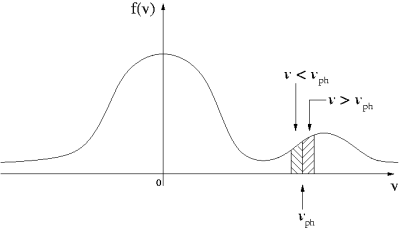
\includegraphics[scale=0.7]{4.png}
\end{center}

\end{document}